\subsection{Configuration générale}
\begin{itemize}
    \item Contrôler le nom d'hôte et de domaine (figure \ref{fig:04-configuration-generale-01})
    \item Renseigner les serveurs DNS et les noms d'hôtes associés (vérification TLS) (figure \ref{fig:04-configuration-generale-02})
    \item Renseigner le fuseau horaire et les serveurs de temps (figure \ref{fig:04-configuration-generale-03})
\end{itemize}

\begin{tip}
    Au moins trois références de temps devraient être utilisées. Les références suivantes peuvent être utilisées:
    \begin{itemize}
        \item \textbf{pool.ntp.org}
        \item \textbf{time.nist.gov}
        \item \textbf{time.google.com}
        \item \textbf{pfsense.pool.ntp.org}
        \item \textbf{time.windows.com}
    \end{itemize}
\end{tip}

\begin{figure}[H]
    \centering
    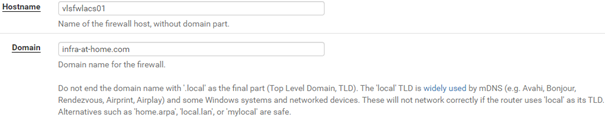
\includegraphics[width=1.0\textwidth]{04-Configuration/Images/04-configuration-generale-01.png}
    \caption{Configuration - Générale - Nom d'hôte et de domaine}
    \label{fig:04-configuration-generale-01}
\end{figure}

\begin{figure}[H]
    \centering
    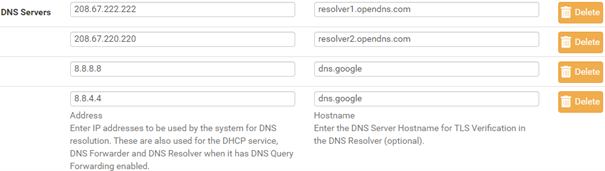
\includegraphics[width=1.0\textwidth]{04-Configuration/Images/04-configuration-generale-02.png}
    \caption{Configuration - Générale - Serveurs DNS}
    \label{fig:04-configuration-generale-02}
\end{figure}

\begin{figure}[H]
    \centering
    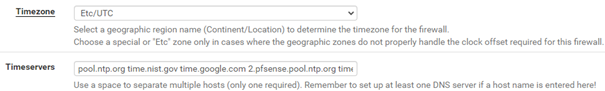
\includegraphics[width=1.0\textwidth]{04-Configuration/Images/04-configuration-generale-03.png}
    \caption{Configuration - Générale - Fuseau horaire et serveurs de temps}
    \label{fig:04-configuration-generale-03}
\end{figure}